\section{平面三角形}

\begin{theorem}
三角形内角和为\(\pi\).
\begin{proof}
设有\(\triangle ABC\).
过点\(C\)作平行于线段\(AB\)的直线\(PQ\).

由内错角相等,有\begin{equation*}
\angle{PCA} = \angle{CAB}, \quad \angle{QCB} = \angle{CBA},
\end{equation*}又由\(\angle{PCA}+\angle{ACB}+\angle{QCB}=\pi\),可得\begin{equation*}
\angle{CAB}+\angle{ACB}+\angle{QCB}=\pi.
\qedhere
\end{equation*}
\end{proof}
\end{theorem}

\begin{theorem}[正弦定理]
设任意三角形\(\triangle ABC\)的外接圆半径为\(R\),则\begin{equation}
\frac{a}{\sin A}
= \frac{b}{\sin B}
= \frac{c}{\sin C}
= 2R.
\end{equation}
\end{theorem}

\begin{theorem}[余弦定理]
设任意三角形\(\triangle ABC\),有\begin{equation}
c^2 = a^2 + b^2 - 2ab \cos C.
\end{equation}
\end{theorem}
可以看出,勾股定理是余弦定理的特殊情况,即当\(C = \frac{\pi}{2}\)时,有\(\cos C=0\),于是\(c^2 = a^2 + b^2\).

\begin{theorem}[摩尔外德公式]
%@see: https://arxiv.org/pdf/1808.08049.pdf
设任意三角形\(\triangle ABC\),则\begin{gather}
	\frac{a+b}{c}
	= \frac{\cos[(A-B)/2]}{\sin(C/2)}, \\
	\frac{a-b}{c}
	= \frac{\sin[(A-B)/2]}{\cos(C/2)}.
\end{gather}
\end{theorem}

\begin{theorem}[正切定理]
设任意三角形\(\triangle ABC\),有\begin{equation}
\frac{a-b}{a+b} = \frac{\tan[(A-B)/2]}{\tan[(A+B)/2]}.
\end{equation}
\end{theorem}

\section{圆}
\subsection{圆的概念}
\subsection{圆的性质}
\subsection{圆的周长\ 圆周率}
\begin{definition}
定义:圆的周长\(C\)与其直径\(2R\)之比称为\DefineConcept{圆周率},记作\(\pi\),即\begin{equation*}
\pi = \frac{C}{2R}.
\end{equation*}
\end{definition}
由于圆周率是一个常数,那么已知圆的直径(或半径)可以求得圆的周长,而已知圆的周长可以求得圆的直径(或半径).

\begin{property}
给定圆上任意一段弧,若它的角度为\(\theta\),那么弧长为\(\theta r\).
\end{property}

\begin{corollary}
如下图,在单位圆上,当圆弧的角度\(\theta\)为锐角,即\(0<\theta<\pi/2\)时,\(\theta > x\). \begin{center}
\begin{tikzpicture}[scale=4]
%\draw[help lines, color=gray!30, dashed] (0,0) grid (1,1);
\pgfmathsetmacro{\u}{sqrt(3)/2}
\coordinate (O) at (0,0);
\coordinate (A) at (\u,0);
\coordinate (B) at (\u,1/2);
\draw (1,0)arc[start angle=0,end angle=30,radius=1]node[midway,right]{\(\theta\)} -- (0,0)node[midway,above left]{\(1\)} -- (1,0)
	(A) -- (B)node[midway,left]{\(x\)};
\draw pic["\(\theta\)",draw=orange,-,angle eccentricity=1.7,angle radius=5mm]{angle=A--O--B} pic[draw=gray,-,angle radius=0.3cm]{right angle=B--A--O};
\end{tikzpicture}
\end{center}
\end{corollary}

\section{平面凸多边形}
\begin{theorem}
设凸多边形的边数为\(n\),则其内角和为\((n-2)\pi\).
\end{theorem}
如图,在凸多边形内部任取一点\(P\),连接该点与凸多边形各顶点,可以得到\(n\)个三角形.
因为三角形内角和为\(\pi\),所以\(n\)个三角形内角和的总和为\(n\pi\),
再减去各三角形\(\angle P\)之和\(2\pi\),可知凸\(n\)边形的内角和为\((n-2)\pi\).
\begin{figure}[htb]
	\centering
	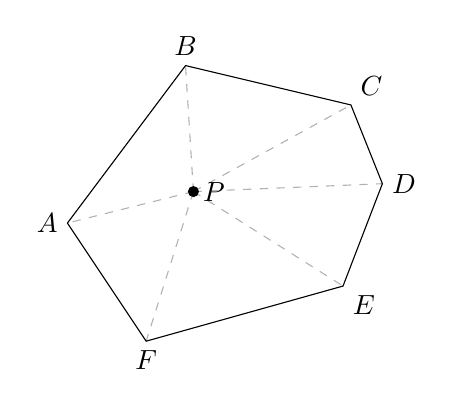
\begin{tikzpicture}
		\coordinate (A1) at (0,2);
		\coordinate (A2) at (1.5,4);
		\coordinate (A3) at (3.6,3.5);
		\coordinate (A4) at (4,2.5);
		\coordinate (A5) at (3.5,1.2);
		\coordinate (A6) at (1,0.5);
		\coordinate (P) at (1.6,2.4);
		\draw[dashed,color=black!30] (P)--(A1) (P)--(A2)
			(P)--(A3) (P)--(A4) (P)--(A5) (P)--(A6);
		\draw (A1)node[left]{\(A\)}--(A2)node[above]{\(B\)}
			--(A3)node[above right]{\(C\)}
			--(A4)node[right]{\(D\)}
			--(A5)node[below right]{\(E\)}
			--(A6)node[below]{\(F\)}--(A1)
			(P)node[right]{\(P\)};
		\fill (P)circle(2pt);
	\end{tikzpicture}
	\caption{}
\end{figure}

\begin{theorem}
凸多边形的外角和为\(2\pi\).
\end{theorem}

\section{凸多面体}
\begin{theorem}[欧拉公式]
设凸多面体的顶点数、棱数、面数分别为\(V\)、\(E\)、\(F\),则有\begin{equation*}
	V - E + F = 2.
\end{equation*}
\end{theorem}

\begin{definition}
\DefineConcept{正凸多面体}(简称\DefineConcept{正多面体}),
是指满足以下条件的凸多面体:
\begin{enumerate}
	\item 正多面体的面由正多边形构成;
	\item 正多面体的各个顶角相等;
	\item 正多面体的各条棱长相等.
\end{enumerate}
\end{definition}

\begin{corollary}
正凸多面体只有5种:三四面体、正方体、正八面体、正十二面体、正二十面体.
\end{corollary}
